\documentclass[conference]{IEEEtran}
\IEEEoverridecommandlockouts
% Uncomment the line above if funding identification is required.
% Template version as of 6/27/2024
\usepackage{hyperref}
\usepackage{cite}
\usepackage{amsmath,amssymb,amsfonts}
\usepackage{algorithmic}
\usepackage{graphicx}
\usepackage{textcomp}
\usepackage{xcolor}
\usepackage{booktabs}  % For professional table formatting
\usepackage{adjustbox} 
\usepackage{array}

\def\BibTeX{{\rm B\kern-.05em{\sc i\kern-.025em b}\kern-.08em
    T\kern-.1667em\lower.7ex\hbox{E}\kern-.125emX}}
    
\begin{document}

\title{Kabul - Code Translation}

\author{
\IEEEauthorblockN{Tobias Konieczny}
\IEEEauthorblockA{
\textit{Department of Computer Science} \\
\textit{Technical University of Munich} \\
Munich, Germany \\
tobias.konieczny@tum.de}
\and
\IEEEauthorblockN{Anne Yang}
\IEEEauthorblockA{
\textit{Department of Computer Science} \\
\textit{Technical University of Munich} \\
Munich, Germany \\
anne.yang@tum.de}
\and
\IEEEauthorblockN{Malek Elfhaiel}
\IEEEauthorblockA{
\textit{Department of Computer Science} \\
\textit{Technical University of Munich} \\
Munich, Germany \\
ge65hal@tum.de}
\and
\IEEEauthorblockN{Eric Yiyang Meng}
\IEEEauthorblockA{
\textit{Department of Computer Science} \\
\textit{Technical University of Munich} \\
Munich, Germany \\
ge87nur@mytum.de}
}

\maketitle

\begin{abstract}
This report summarizes the development and evaluation of a code-to-code translation model 
conducted as part of the TUM lab course "Next-Gen Programming: AI-Powered Software Programming with Deep Learning.". 
The project aimed to fine tune a pre-trained transformer model and making it capable of translating source code between different coding languages.
Additional tasks included data generation, preprocessing, hyperparameter optimization, model evaluation, and benchmarking.
The primary goal was to improve the performance of pre-trained models in terms of translation capability through fine-tuning.
Furthermore, the project included the design and implementation of a web application that allows users to input code snippets and receive their translated equivalents as output.
The web application was successfully deployed and is accessible online at \url{https://code-translation.com}.

The evaluation results demonstrate that fine-tuning pre-trained models with a curated dataset of code snippets can significantly improve their translation performance.
\end{abstract}

\begin{IEEEkeywords}
fine-tuning, code-to-code translation, transformer models, dataset generation, model evaluation.
\end{IEEEkeywords}

\section{Introduction}
In the scope of the lab course we were tasked to find a use case related to prompt-based code generation 
and create an application for it, which leverages the power of transformer models.
During the preliminary requirements elicitation phase, we identified the task of code-to-code translation as a suitable task for this project.

\subsection{Motivation}
Programming languages are one of the most important foundations of software development, enabling developers to create applications across various domains.
However, the constantly growing number of programming languages and frameworks poses a challenge for novices and causes problems related to interoperability of code across different ecosystems.
Thus, the ability to translate code between different programming languages can significantly improve software development workflows, 
facilitate migration between languages, and enhance cross-language compatibility.

\subsection{Objective}
This project aimed to develop a model competent of code-to-code translation by leveraging pre-trained transformer models.
The primary objective was to fine-tune pre-trained models on a curated dataset of code snippets 
to improve their translation capability.
Additionally, the project involved designing and implementing a web application to provide a user-friendly interface for real-time code translation.

\subsection{Core Contributions}
\begin{itemize}
\item The creation of balanced datasets for fine-tuning and evaluation of the models, ensuring high code quality of the code snippets. 
\item The fine-tuning of transformer-based models for code-to-code translation, achieving significantly better performance compared to the baseline pre-trained models.
\item A comprehensive evaluation of the fine-tuned models using metrics such as the ROUGE-, BERT-, FRUGAL-, and TER-Score as well as manual benchmarking to demonstrate their performance.
\item The implementation of a web application enabling users to input code snippets and receive translated output.
\end{itemize}

The report is organized in the following manner:
Section \ref{dev} details the software development process and implementation of the web application. Including frontend and backend modelling and implementation as well as the process of containerization and the web deployment of the web application.  
Section \ref{train} details the training process, including model selection, dataset-research, -creation and -preprocessing as well as fine-tuning strategies.
Section \ref{eval} presents the evaluation and benchmarking process and results, as well as their implications.
Section \ref{learn} highlights key lessons learned during the project, and section \ref{conc} concludes with a summary of outcomes and the final product.

\section{Software Development Process}\label{dev}
\subsection{Overview}
The software development process encompasses several key components. 
This section provides a detailed explanation of the methodologies employed in developing the frontend and backend as well as some implementation specifics. It also covers the steps taken for containerization and the subsequent deployment of the application, ensuring accessibility and usability for end-users.
The source code can be found at \cite{b1}.

\subsection{Frontend}
This section will detail the frontend development process. It includes a comprehensive overview of the design choices made, and the continuous improvements made throughout the iterative development phases of our software implementation process.

Following the preliminary requirements elicitation the first step of our development process was drafting a design for the user interface. After an initial sketch drawing on a whiteboard a more detailed specification of the design using Figma was performed.
Thereupon, the process of the implementation for the first version of the user interface began.
We decided to use the React library to create our user interface. Main reasons for choosing React were its component-based architecture, which improves code reusability and maintainability, and its efficient virtual Document Object Model (DOM) implementation, which optimizes performance, resulting in a smother user experience and easier scalability of applications.   

Our frontend development progressed through three distinct versions, each introducing new features and enhancements tailored to meet evolving project requirements and user needs.

\begin{enumerate}
    \item \textbf{Version 1}
    \begin{itemize}
        \item \textbf{Features}: Initially focused on core functionality, Version 1 included basic user interface elements for code input and output as well as input and output language selection. It also featured basic buttons for uploading code input, copying the resulting output, saving the resulting output in a .txt file and a button for the initiation of the translation process. The translation button was connected to the backend \ref{backend} which at that stage only supported a pre-trained baseline-model not capable of any acceptable translation. A detailed explanation of the models can be found in section \ref{train-model}.
        \item \textbf{Purpose}: Primarily aimed at establishing foundational capabilities and validating basic functionality.
    \end{itemize}
    
    \item \textbf{Version 2}
    \begin{itemize}
        \item \textbf{Features}: Minor changes in button design and the design of the code input and output boxes. This version also featured correct file endings when downloading the resulting translations. Additionally, response streaming was implemented, which allows text output to be delivered progressively as it is generated, rather than waiting for the entire response to finish. Accompanied with these features came the restriction to only support the programming languages Java, Python and C++, which is reasoned in section \ref{data}. Moreover, this version was able to perform acceptable translations due to first successes in model fine-tuning \ref{fine-tuning}. 
        \item \textbf{Purpose}: Focused on base functionality and design improvements.
    \end{itemize}
    
    \item \textbf{Version 3}
    \begin{itemize}
        \item \textbf{Features}: Includes an example problem section, which allows users to try out the functionality of the web application with predefined code snippets. It additionally includes a button to switch between light-mode and dark-mode as well as the functionality to initiate the translation via the key combination Ctrl+Enter.
        \item \textbf{Purpose}: Iteratively refined to enhance user experience.
    \end{itemize}
\end{enumerate}


\subsection{Backend}\label{backend}
In this section, the interaction between frontend components and backend services, and the integration of the fine-tuned model into the Django backend of the project will be discussed. The integration of the model forms a critical component of the system's functionality, enabling seamless translation capabilities through a user-friendly frontend.

Using the Django framework for the backend, specifically the Django REST Framework (DRF), simplifies API development, ensuring efficient data transfer and seamless interaction between frontend components and backend services. 
The code translation process forms the only interaction between frontend components and backend services. This interaction is implemented through a POST request to the backend server from the frontend. The POST request includes the input code, which should be translated, as well as the programming language it is written in and the target output programming language. This triggers the translation process and subsequently the StreamingResponse from the backend server, ideally including the translated equivalent.

The main part of the backend forms the integration of the fine-tuned model. 
The backend utilizes the HuggingFace Transformers library to integrate the fine-tuned model. Specifically, the T5ForConditionalGeneration model type is used to translate code between programming languages. Upon receiving a POST request with the code and language details, the backend processes the input and initiates the model's code generation process in a separate thread to maintain responsiveness. The translated code is streamed back to the frontend using a StreamingHttpResponse, providing real-time feedback to the user.


Taking advantage of the HuggingFace Transformer library and the DRF, the backend setup manages to efficiently combine the interaction between the frontend and the backend with the integration of the fine-tuned model, responsible for the code translation process. 

\subsection{Containerization}
During the development of the project, Docker was used to containerize both frontend and backend. Major advantage of the containerization is the isolation of each component with its dependencies in a Docker container, guaranteeing identical behaviour across different environments and eliminating common setup discrepancies. 
Being able to easily deploy the software locally, independent of the local operating system, simplified the software development process greatly. Especially taking advantage of the functionalities provided by docker compose, enabling simultaneous deployment of the frontend and backend server, ensured a faster development and changes working consistently across all development environments. 

\subsection{Deployment}
The final step of the software development process, was the deployment of the containerized frontend and backend. 
For this step, Google Cloud Run Services was chosen. 
Using Google Cloud Run Services came with many benefits.
It supports automatic scaling, thus automatically adjusting the number of container instances based on incoming traffic, ensuring smooth usability. Moreover, it is a pay-as-you-go pricing model, ensuring costs for only those resources used by the deployed containers, thus reducing costs during idle periods. 
This fully managed service, Google Cloud Run provides, handles all aspects of server management, updates and scaling, allowing our web application to be publicly accessible.

\section{Fine-tuning Process}\label{train}
The development of an effective code-to-code translation model requires a structured fine-tuning process to optimise translation accuracy. This section describes the specific aspects of fine-tuning, including the process behind model selection, dataset research, and the fine-tuning strategies employed to improve performance.

\subsection{Hardware Restrictions}
The training of deep learning models requires computational resources. Thus, due to hardware restrictions, the approach was optimized by utilizing more accessible resources, such as Google Colab's T4 GPU, which offers 2 hours and 30 minutes of free daily computational time, and a home GPU setup (GPU: GeForce RTX 2070 SUPER MINI).
These restrictions had a significant impact on model selection, dataset size, and the fine-tuning process. The following sections detail the strategies we employed to address these challenges effectively.

\subsection{Model Selection}\label{train-model}
Selecting an appropriate model was an important step in ensuring quality code-to-code translation while maintaining efficiency within the hardware restrictions. Given the limited computational resources, the focus was on two aspects. Firstly, models that could understand code, but were ineffective at code translation tasks. And secondly, models that could be fine-tuned on the available hardware.

To identify suitable models, research was primarily conducted on Hugging Face's Model Hub \cite{b2}, where transformer-based architectures designed for code-related tasks were analyzed. The main selection criteria were model size, computational efficiency and how easy integration was. Based on these considerations, the following seven transformer models were selected.

Salesforce/codeT5-small (T5S) \cite{b3} was chosen as a lightweight version of CodeT5 with approximatedly 60 million parameters, specifically optimised for code-related tasks. Its small parameter size made it particularly well suited for training on the limited hardware. It allowed for faster fine-tuning and a stronger performance.

To complement this, Salesforce/codeT5-base (T5B) \cite{b4} was selected as a more powerful variant of CodeT5, which had approximately 220 million parameters.

A further baseline included (GPT2) \cite{b5}, a general purpose language model with 137 million parameters originally designed for text generation but capable of processing code. Although not specifically optimised for programming languages, this model served as a benchmark to evaluate how a non-code-specific transformer performs in code translation tasks.

In addition, microsoft/codebert-base (CodeBERTB) \cite{b6} was included, a model pre-trained on a mixture of natural language and source code with 125 million parameters, due to its generally strong performance on code-related tasks.

Another model in the selection was NousResearch/Llama-3.2-1B (Llama1B) \cite{b7}, a compact version of the LLaMA architecture optimised for both natural language and code tasks with 1.24 billion parameters. This model was considered as an alternative to larger, more resource-intensive transformers, ensuring that a computationally feasible option was provided while still benefiting from the advanced capabilities of LLaMA. However, during the actual fine-tuning process we noticed that due to the before mentioned hardware restrictions, fine-tuning duration would take longer than our hardware could manage. Thus, Llama1B was excluded from fine-tuning and evaluation.  

For further evaluation, facebook/bart-base (BARTB) \cite{b8} was included, a sequence-to-sequence transformer model designed for text and code generation with 139 million parameters. This model provided an additional basis for assessing the effectiveness of transformer-based approaches in translation tasks.

Finally, alirezamsh/small100 (SMALL100) \cite{b9}, a slimmed version of the M2M-100 model optimised for multilingual and code translation with 333 million parameters, was chosen to analyse its efficiency in handling different programming language constructs. This model allowed for the investigation of whether a smaller-scale multilingual approach could be competitive in code translation tasks.

Given the before mentioned hardware constraints, models with fewer parameters were prioritised to reduce memory requirements and training time. 

\subsection{Dataset Research}\label{data}
As clean data is remarkably important in order to increase predictive accuracy of pre-trained models, thorough research was conducted to construct a qualitative and balanced dataset. 
The initial finding process involved conducting research until the two datasets, NTU-NLP-sg/xCodeEval (NTU) \cite{b10} and ziwenyd/transcoder-geeksforgeeks (G) \cite{b11}, were categorized as suitable. Fine-tuning the first models, Salesforce/codeT5-small and Salesforce/codeT5-base, on both datasets respectively highlighted the necessity of versatile and clean data. This lead to the iterative construction of different dataset versions to improve translation quality. As the project progressed, the six other models were included and fine-tuned on the four datasets mentioned below. 
This was done to increase translation performance and diversify the fine-tuning process.

\begin{itemize}
    \item \textbf{Version 1 (V1)}
        
        Version 1 consists of the NTU-NLP-sg/xCodeEval and the ziwenyd/transcoder-geeksforgeeks dataset. The merged dataset of both served as a foundational resource for code examples and consists of 50717 code pairs and four columns: Input Language, Input Code, Output Language, and Output Code. 
    
    \item \textbf{Version 2 (V2)}
        
        In this version, an emphasis was placed on increasing the code quality and thus decreasing the dataset size. To achieve better code quality, CodexGlue \cite{b12}, a dataset  dominated by C\# and Java code, was included. Additionally, code pairs were generated using ChatGPT to expand the available translations. The columns did not change to the previous version, although the dataset size decreased to 23007 code pairs.
    
\end{itemize}

The focus of the first two versions of the datasets was purely quantitative. Therefore, eleven programming languages were included in the first two versions, including Java, Python, C, C++, C\#, Rust, etc. Naturally, code quality suffered. 
So, in subsequent versions of the dataset, the focus shifted to balance and quality. For this reason, the number of languages was reduced to three: Java, Python and C++, as the functionality of these languages is similar.

\begin{itemize}
    \item \textbf{Version 3 (V3)} 
        
        Here, web scraping was employed to extract high-quality solutions from LeetCode \cite{b13}. It ensured that the dataset contained diverse and well-structured problem-solving code.
        The dataset structure differs from the first two versions. This dataset includes 500 functions, which make 3000 code pairs among three columns: Java, Python, and C++.

    \item \textbf{Version 4 (V4)}
        
        Finally, additional code pairs from GeeksforGeeks were added, further refining the dataset’s structure and ensuring a wider coverage of programming functions.
        The columns did not change to V3, however the dataset size increased. It includes 1045 functions among three languages, which make up 6270 code pairs.
    
\end{itemize}

To prevent excessive training times, the dataset size was reduced by  selecting a subset of high-quality code snippets while ensuring diversity in programming constructs. All datasets were saved as Comma-Separated Values (CSV) files.

\subsection{Fine-Tuning Process}\label{fine-tuning}
In order to fine-tune the pre-trained models on the code translation use case, the following fine-tuning steps were taken. With the help of the Hugging Face Library, the fine-tuning process was streamlined, which made efficient model adaptation possible. The procedure consisted of the following steps.
Firstly, the dataset was loaded from CSV files and converted into a structured format suitable for training. Secondly, the data was split into training, test, and validation sets to properly evaluate the model. Then, the transformer model was initialized using the Hugging Face Transformers library and tokenization and encoding were applied in order to preprocess the values, contained in the dataset, into a format, that was compatible with the model's transformer architecture. As the dataset structure in V1 and V2 differs from V3 and V4, preprocessing data was also different. Lastly, the training arguments, i.e. hyperparameters, such as learning rate, batch size, number of epochs, etc. were defined and the model was then fine-tuned. 
To increase training efficiency and combat hardware restrictions, certain strategies were employed:

\begin{itemize}
    \item \textbf{Low Rank Adaption (LoRA)} 
        
        To optimize the fine-tuning process, Low-Rank Adaptation (LoRA) was employed. LoRA is a technique that leverages low-rank decomposition to train smaller matrices instead of updating all model parameters. The pre-trained model weights are frozen and LoRA-specific smaller matrices are introduced and trained. Once optimized, these LoRA weights are transformed and added to the pre-trained model parameters.   

    \item \textbf{Model Quantization}
        
        Another strategy employed to optimize the fine-tuning process was Model Quantization. This technique reduces the computational and memory costs of inference by presenting model weights from higher bits precision to lower bits precision, e.g. leveraging an 8-bit-integer over a 32-bit-floating point.

    \item \textbf{Early Stopping}

        Early stopping was utilized in the fine-tuning process as a regularization technique, which prevents overfitting. Based on predefined criteria regarding the number of epochs after which the model begins to become weaker in generalization, the method monitors the model's performance and automatically stops the training process once no further improvement is detected.
        
    \item \textbf{Hyperparameters}

        In order to combat the hardware restrictions within the training arguments, the number of epochs was decreased to numbers smaller than 30. It became apparent that larger batch sizes implied shorter training times, and vice versa. However, using excessively large batch sizes increased RAM requirements, limiting training efficiency. The batch size was varied depending on the hardware resources for the fine-tuning.
        In comparison to the influence the before mentioned datasets had on the output, the influence of varying learning rates could be neglected. 
        
   
\end{itemize}

\section{Evaluation and Benchmarking}\label{eval}
To assess the fine-tuned models after the fine-tuning process, we implemented an automatic evaluation script that employs several evaluation metrics and benchmarked chosen examples manually. 
This section explains the benchmarking approach and \ref{res} discusses the results. All related scripts and excel files are available in \cite{b1}.

\subsection{Metrics and Automatic Benchmarking Approach}
We used the following metrics for a combination of lexical, edit-distance, and semantic similarity metrics to ensure a broad and complementary evaluation:
\\
\textbf{ROUGE-1, ROUGE-2, ROUGE-L, ROUGE-Lsum} – Measures n-gram overlap, a continuous sequence of n words, between generated and reference code. A higher score close to 1 indicates better performance
    \begin{itemize}
        \item Rouge 1: Overlap of unigrams
        \item Rouge 2: Overlap of bigrams
        \item Rouge-L: Longest common subsequence
        \item RougeLsum: Similar to Rouge-L on a summary level
    \end{itemize}
\textbf{TER (Translation Edit Rate)} – Calculates the number of edits required to transform the generated output into the reference. A lower TER score indicates better code generation accuracy \cite{b14}.
\\
\textbf{BERTScore} – Evaluates the semantic similarity between the generated and reference code. It consists of:  
\begin{itemize}
    \item  Precision: Measures how much of the generated output is relevant to the reference.  
    \item  Recall: Measures how much of the reference is captured in the generated output.  
    \item F1 Score: Combines both Precision and Recall for a balanced assessment. 
\end{itemize}
For our visualization, we used the F1 Score as a reference for the quality of code generation in terms of functionality. A value close to 1 indicates better performance \cite{b15}.
\\
\textbf{FrugalScore} - A lightweight alternative to BertScore
\\\\
These metrics are computed in a script using the evaluate library from Hugging Face \cite{b16}. We evaluated the overall performance with a reference dataset that includes 150 code pairs (Overall benchmark dataset) from the V4 dataset which we excluded from the training process. Furthermore, the performance of each model on each specific translation task (e.g. Python to Java, Java to C++, etc.) was also evaluated with a set of 25 code pairs per task. The results were exported to an excel spreadsheet, to be later loaded by a visualization script to visualize the key findings which are presented in \ref{res}.


\subsection{Manual Benchmarking Approach}
As automatic metrics lack in assessing qualitative aspects, such as logical accuracy or adherence to coding standards, manual benchmarking was additionally performed.
Here, we used the following six fundamental programming functions: the Factorial function, checking if a number is prime, reversing a string, the Fibonacci function, finding the greatest common divisor, and a main function printing "Hello world". All possible translation pairs were tested and the generated output was compared against reference implementations stored in an excel spreadsheet \cite{b1}.
\subsection{Results}\label{res}

\subsubsection{Automated Metric Comparison}
Table \ref{tab:comp} presents all computed metrics, evaluated on the overall benchmark dataset, for both the baseline models and the best fine-tuned model respectively. Our fine-tuned models show almost consistent improvements across all evaluation metrics. These improvements indicate that fine-tuning enhances both the syntactic and semantic accuracy of the generated code. One exception to this trend was CodeBERTB, which showed a decline in performance compared to the baseline model. This could be attributed to its architecture, which is less suited for sequence-to-sequence tasks like code translation, than the architecture of  the other models. A more detailed analysis on the difference is provided below.
    \begin{figure}[htbp]
\centerline{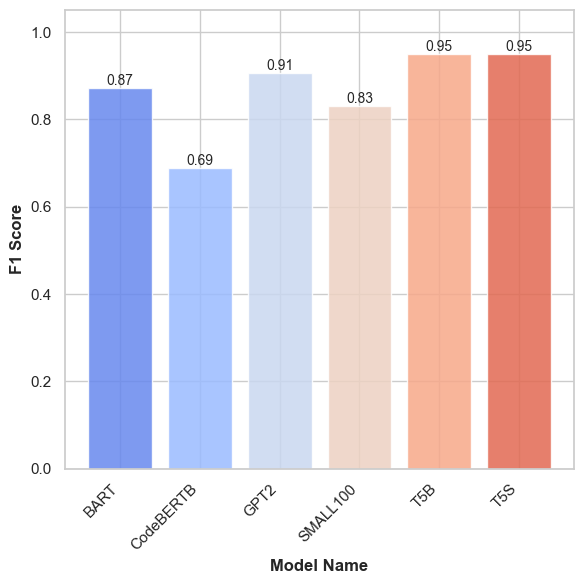
\includegraphics[width=\columnwidth]{images/final.png}}
\caption{Best fine-tuned versions of all baseline models}
\label{overall}
\end{figure}
\begin{table*}[h]
    \caption{Comparison of Baseline vs. Fine-Tuned Model Metrics Overview}
    \label{tab:comp}
    \renewcommand{\arraystretch}{1.5} 
    \resizebox{\textwidth}{!}{  % Ensures table fits within page width
    \begin{tabular}{lccccccc}
        \toprule
        \textbf{Model} & \textbf{ROUGE-1} & \textbf{ROUGE-2} & \textbf{ROUGE-L} & \textbf{ROUGE-Lsum} & \textbf{TER ↓} & \textbf{BERT F1} & \textbf{FrugalScore} \\
        \midrule
        CodeT5-Base (Baseline Model) & 0.17 & 0.05 & 0.15 & 0.16 & 96.44 & 0.79 & 0.50 \\
        
        CodeT5-Base (Best Fine-Tuned) & 0.76 & 0.65 & 0.72 & 0.76 & 53.02 & 0.95 & 0.90 \\
        
        CodeT5-Small (Baseline Model) & 0.07 & 0.01 & 0.06 & 0.07 & 97.16 & 0.74 & 0.44 \\
        
        CodeT5-Small (Best Fine-Tuned) & 0.77 & 0.67 & 0.74 & 0.77 & 46.38 & 0.95 & 0.89 \\
        
        GPT-2 (Baseline Model) & 0.40 & 0.27 & 0.37 & 0.40 & 232.78 & 0.86 & 0.65 \\
        
        GPT-2 (Best Fine-Tuned) & 0.65 & 0.45 & 0.61 & 0.65 & 67.76 & 0.91 & 0.66 \\
        
        BART (Baseline Model) & 0.41 & 0.19 & 0.34 & 0.39 & 136.31 & 0.83 & 0.54 \\
        
        BART (Fine-Tuned) & 0.61 & 0.38 & 0.57 & 0.61 & 93.02 & 0.87 & 0.66 \\
        
        CodeBERT (Baseline Model) & 0.00 & 0.00 & 0.00 & 0.00 & 100.68 & 0.69 & 0.32 \\
        
        CodeBERT (Fine-Tuned) & 0.00 & 0.00 & 0.00 & 0.00 & 288.89 & 0.67 & 0.32 \\
        
        Small100 (Baseline Model) & 0.00 & 0.00 & 0.00 & 0.00 & 100.37 & 0.71 & 0.31 \\
        
        Small100 (Fine-Tuned) & 0.26 & 0.14 & 0.24 & 0.24 & 92.37 & 0.83 & 0.63 \\
        
        \bottomrule
    \end{tabular}
    }
    \label{tab:base_vs_finetuned}
\end{table*}
\begin{itemize}
    \item \textbf{ROUGE Scores}: The fine-tuned models achieved higher ROUGE-1, ROUGE-2, ROUGE-L, and ROUGE-Lsum scores compared to the baseline models, indicating better n-gram overlap between the generated output and the reference. The highest average improvement among all Rouge Scores by a factor of 25 was achieved with the fine-tuning of the pre-trained CodeT5-Small model.
    \item \textbf{Translation Edit Rate (TER)}: Observing the results of the TER scores shows that fine-tuning the models significantly lowers the respective TER scores. The fine-tuning of the GPT2 model resulted in an improvement of about 70\% and both CodeT5 models improved by about 50\%. This demonstrates that fewer edits are required to transform the translated code into the reference implementation.
    \item \textbf{BERTScore}: The fine-tuned models display improvements in BERTScore, reflecting better semantic alignment with the reference code. This is especially important for preserving the meaning of the code during translation. As shown in Fig. \ref{overall}, all our fine-tuned models, except CodeBERTB, reached a F1 Score above 0.80. Notably, both T5-based models reached a score of around 0.95 which is almost an ideal value of 1.
    \item \textbf{FrugalScore}:
    The trends mentioned above can be confirmed with the Frugal Score as well. Here, the fine-tuned versions of Small100 and the T5 Models have the most noticeable value improvement of about 103\% and 100\%
    \end{itemize}

Furthermore, the benchmarking results of the specific code pairs showed similar developments. Some noticeable observations are the translation from Java to C++ and Java to Python. Here, the F1 Score reached a value over 0.95 for the T5 models. 

\subsubsection{Focused analysis on Top-Performing Models}
Based on the overall benchmarking results, we identified the three top-performing models:
\begin{itemize}
    \item \textbf{Model 1}: CodeT5-Small trained with V4
    \item \textbf{Model 2}: CodeT5-Base trained with V4
    \item \textbf{Model 3}: CodeT5-Small trained with V2
\end{itemize}
To gain deeper insights, we analyzed the three top-performing models along with their respective baseline models. For a clear evaluation, we used the BERT-F1 score, as it is a strong indicator of the semantic quality of the generated translations \cite{b15}.

\begin{itemize}

    \item\textbf{CodeT5 Small} (Baseline Model of Model 1 and Model 3):
    The baseline model initially achieved scores of TER = 97.16, F1 = 0.74, all Rouge Scores below 0.1, and a Frugal Score of 0.44. After fine-tuning, the best-performing model demonstrated significant improvements: TER decreased by approximately 52\%, F1 increased by around 28\%, Rouge Scores improved by a factor of 25, and the Frugal Score saw an enhancement of roughly 102\%.

    Fig. \ref{small} illustrates the performance development across our datasets. The model fine-tuned on dataset V4 had the best performance, indicating that our balanced dataset enhanced the fine-tuning process. Model 3 also showed notable improvements, suggesting that dataset quality, balance and size are crucial factors in model performance.
    \item \textbf{CodeT5 Base }(Baseline Model of Model 2)
    The baseline model started with the following scores: TER = 96.44, F1 = 0.79, all Rouge Scores under 0.2, and FrugalScore = 0.50.
    Fine-tuning on the V4 dataset resulted in the second-best performing model, with TER reduced by approximately 45\%, F1 increased by around 20\%, ROUGEScores improved by a factor of 7, and FrugalScore reaching an improvement of 80\%. As illustrated in Fig. \ref{base}, similar to CodeT5 Small, the V4 dataset outperformed other datasets. Additionally, the model trained on the G dataset, which is partially included into V4, also has a high score of 0.92. This shows the effectiveness of our V4 dataset for fine-tuning. 

\end{itemize}

\begin{figure}[htbp]
\centerline{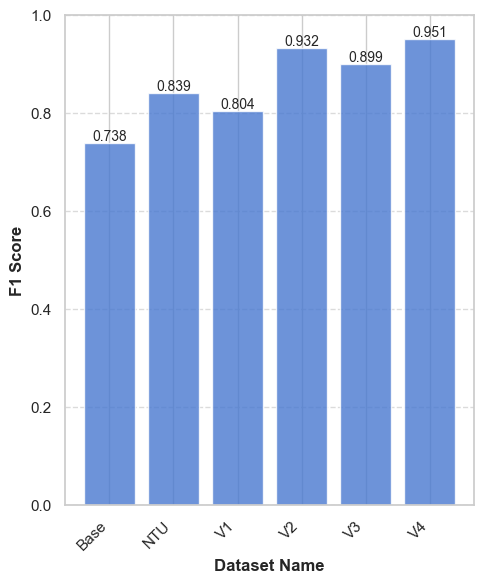
\includegraphics[width=\columnwidth]{images/t5_small.png}}
\caption{F1 Score comparison of CodeT5-Small across different datasets}
\label{small}
\end{figure}


\begin{figure}[htbp]
\centerline{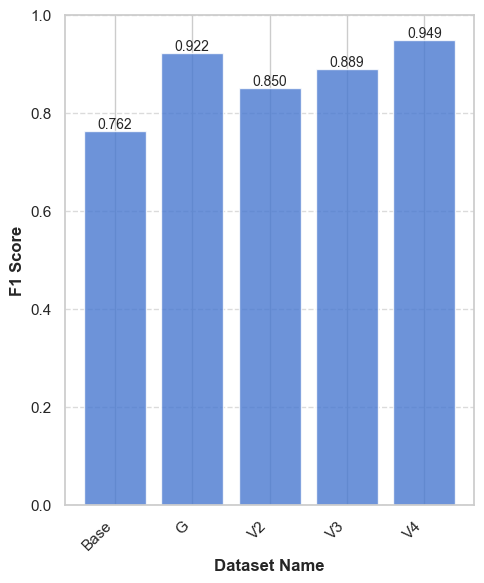
\includegraphics[width=\columnwidth]{images/t5_base.png}}
\caption{F1 Score comparison of CodeT5-Base across different datasets}
\label{base}
\end{figure}

\subsubsection{Manual Benchmarking Results}
In addition, we conducted manual benchmarking, as standard metrics have their limitations. 

\begin{itemize}
    \item \textbf{CodeT5-Small} (Baseline Model): 
    Initially, the baseline model could only generate single characters or one-word outputs, such as `=`, `:`, or simple function names. 
    \item \textbf{CodeT5-Base} (Baseline Model):
    The baseline model produced incomplete and senseless code snippets.
    \item
    \textbf{Observations and Limitations}:
    For Java as the target language, the models tend to import unnecessary libraries and include a class definition instead of a standalone function. We believe this is due to the characteristics of the training datasets. Additionally, for the factorial function translation, Model 2 generates only `import math` as the output. 
    \item \textbf{Strenghts}:
    All three top-performing models are capable of generating nearly correct, functional code. The generated functions generally follow the structure of the respective programming language, maintain basic code formatting, and conceptually align with the expected implementation. Additionally, the models effectively handle all language pairs while distinguishing between Python syntax and Java/C++ syntax, which includes `\{\}` brackets. 
    For further details check the excel files contained in \cite{b1}.
    \\    
\end{itemize}


\subsubsection{Conclusion}
The evaluation demonstrates that our fine-tuning significantly improves model performance across all metrics compared to the baseline model, which was also verified through manual benchmarking.

\section{Lessons Learned}\label{learn}
Throughout the duration of this project, our team gained valuable insights into the domains of machine learning (ML), artificial intelligence (AI), and deep learning. Below, we reflect on the technical knowledge acquired and finally, challenges encountered.

\subsection*{Technical Insights}
\begin{enumerate}

    \item \textbf{Development Processs}: We learned to build a project based on a preliminary requirements elicitation as well as following agile software development processes.

    \item \textbf{Impact of Dataset Quality and Size}: The project highlighted the importance of dataset selection. We observed that both the size and quality of training data directly affect model accuracy and generalization. Smaller or low quality code datasets led to suboptimal translation outputs.

    \item \textbf{Model Fine-Tuning and Hyperparameters}: We developed a comprehensive understanding of fine-tuning pre-trained models, particularly the role of hyperparameters such as learning rate and epochs. Although hyperparamter tuning plays a major part in model training, we observed that altering datasets for the fine-tuning were more significant in our case, as described above.
    
    \item \textbf{Efficiency Techniques}: Implementing LoRA and quantization taught us to manage large datasets effectively, accelerating training while maintaining model performance. These techniques proved invaluable for balancing computational efficiency with resource constraints.
    
    \item \textbf{Evaluation Metrics}: We learned to systematically test our model's translation efficiency using metrics such as BERT Score, ROUGE, and TER. These tools helped quantify the model's strengths and weaknesses. However, we also learned that manual benchmarking is equally important, as these mertrics fail to include qualitative aspects.
    
    \item \textbf{Deployment Challenges}: Deploying the model into a web interface taught us more skills in frontend development, backend integration, and containerization using Docker and Docker Compose. We gained experience in linking these components together to create a website.
\end{enumerate}

\subsection*{Challenges and Limitations}
\begin{itemize}
    \item \textbf{Hardware Constraints}: Limited access to high-performance computing resources posed a little bit of constraint. Fine-tuning large models, even with efficiency techniques like quantization, required prolonged processing times, which delayed experimentation and iteration.
    
    \item \textbf{Trade-offs in Model Complexity}: To accommodate hardware limitations, we occasionally prioritized faster training times over model complexity, potentially sacrificing translation accuracy.
\end{itemize}

\section{Conclusion}\label{conc}
The increasing number of programming languages has made code interoperability a challenge in software development. To combat this challenge, our project focused on fine-tuning a pre-trained transformer-based model in order to achieve an increase in performance of code translation accuracy to the baseline model. By ensuring dataset quality and employing methods, such as LoRA, Quantization, and Early Stopping, we significantly improved translation performance while working within hardware constraints.

The results of our benchmarking and evaluation highlight that fine-tuning pre-trained models on thoroughly prepared datasets of code snippets can significantly increase translation accuracy. A prime example is the Salesforce/codet5-small model, fine-tuned one the V4 dataset, achieving a 0.95 BERT F1 score, which means a 28\% increase compared to the baseline model. However, automated metrics primarily assess lexical and semantic similarities. This implies that evaluating functional correctness with only these metrics remains challenging. To prevent a one-sided evaluation, manual benchmarking was additionally conducted utilizing fundamental programming functions. The combined result of both evaluation methods emphasize that the Salesforce/codet5-small model fine-tuned on dataset V4 performed the best, lexically, semantically, and functionally.

Another goal of this project was to integrate the fine-tuned model into a real-world setting. In this project, it was successfully achieved through the development of a web interface, which can be accessed at \url{https://code-translation.com}. This allows users to interact with our project in real-time. The development process encompassed containerization and cloud-based scalability.

Ultimately, the results of this project highlight the ability of improving task-specific capabilities of baseline models through thorough data preparation and intelligently designed fine-tuning processes.


\begin{thebibliography}{00}

\bibitem{b1} 
T. Konieczny, A. Yang, M. Elfhaiel, E. Y. Meng (2025) Code Translation Model and Web Application [Source Code]. \url{https://gitlab.lrz.de/bpc-ws-2425/kabul}
\bibitem{b2} 
Hugging Face, “Hugging Face Model Hub,” Hugging Face, 2024. [Online]. Available: \url{https://huggingface.co/models}
\bibitem{b3} 
Salesforce, “Salesforce/codeT5-small: Open-source code intelligence model,” Hugging Face, 2024. [Online]. Available: \url{https://huggingface.co/Salesforce/codeT5-small}
\bibitem{b4} 
Salesforce, “Salesforce/codeT5-base: Open-source code intelligence model,” Hugging Face, 2024. [Online]. Available: \url{https://huggingface.co/Salesforce/codeT5-base}
\bibitem{b5}
OpenAI, “openai-community/gpt2: GPT-2 language model,” Hugging Face, 2024. [Online]. Available: \url{https://huggingface.co/openai-community/gpt2}
\bibitem{b6}
Microsoft, “microsoft/codebert-base: A bimodal pre-trained model for code understanding,” Hugging Face, 2024. [Online]. Available: \url{https://huggingface.co/microsoft/codebert-base}
\bibitem{b7}
Nous Research, “NousResearch/Llama-3.2-1B: Lightweight LLaMA model for language and code tasks,” Hugging Face, 2024. [Online]. Available: \url{https://huggingface.co/NousResearch/Llama-3.2-1B}
\bibitem{b8}
Facebook AI, “facebook/bart-base: A sequence-to-sequence transformer model for text and code generation,” Hugging Face, 2024. [Online]. Available: \url{https://huggingface.co/facebook/bart-base}
\bibitem{b9}
A. Mohammadshahi, V. Nikoulina, A. Berard, C. Brun, J. Henderson, and L. Besacier, "SMaLL-100: Introducing Shallow Multilingual Machine Translation Model for Low-Resource Languages," in *Proceedings of the 2022 Conference on Empirical Methods in Natural Language Processing*, Abu Dhabi, United Arab Emirates, Dec. 2022, pp. 8348–8359. [Online]. Available: \url{https://huggingface.co/alirezamsh/small100}
\bibitem{b10}
M. A. M. Khan et al., "xCodeEval: An Execution-based Large Scale Multilingual Multitask Benchmark for Code Understanding, Generation, Translation, and Retrieval," arXiv preprint arXiv:2303.03004, Nov. 2023. [Online]. Available: \url{https://huggingface.co/datasets/NTU-NLP-sg/xCodeEval}
\bibitem{b11}
Z. Y. Dong, "TransCoder GeeksforGeeks Dataset," Hugging Face, 2023. [Online]. Available: \url{https://huggingface.co/datasets/ziwenyd/transcoder-geeksforgeeks}
\bibitem{b12}
S. Lu et al., "CodeXGLUE: A Machine Learning Benchmark Dataset for Code Understanding and Generation," arXiv preprint arXiv:2102.04664, Feb. 2021. [Online]. Available: \url{https://huggingface.co/datasets/CM/codexglue_codetrans}
\bibitem{b13}
LeetCode, “All LeetCode Problems,” LeetCode, 2024. [Online]. Available: \url{https://leetcode.ca/all/problems.html}
\bibitem{b14}
M. A. Chéragui, "Theoretical overview of machine translation," in *Proc. Int. Conf. Web and Information Technologies (ICWIT)*, 2012, pp. 160-169.
\bibitem{b15}
T. Zhang, V. Kishore, F. Wu, K. Q. Weinberger, and Y. Artzi, 
"BERTScore: Evaluating text generation with BERT," 
in *Proc. Int. Conf. Learn. Representations (ICLR)*, Apr. 2020. 
[Online]. Available: \url{https://arxiv.org/abs/1904.09675}
\bibitem{b16}
Hugging Face, "LightEval Metric List," Accessed Feb. 2, 2025. [Online]. Available: \url{https://huggingface.co/docs/lighteval/metric-list}




\end{thebibliography}


\end{document}


